\documentclass[../notes.tex]{subfiles}

\pagestyle{main}
\renewcommand{\chaptermark}[1]{\markboth{\chaptername\ \thechapter\ (#1)}{}}
\setcounter{chapter}{3}

\begin{document}




\chapter{Ions}
\section{Cations}
\begin{itemize}
    \item \marginnote{9/24:}Lecture 5 recap.
    \begin{itemize}
        \item Pericyclic reactions: Concerted reactions with a TS having a cyclic array of atoms and orbitals.
        \item Three models.
        \begin{enumerate}
            \item Woodward-Hoffmann rules: Conservation of orbital symmetry.
            \item Dewar-Zimmerman analysis: Aromatic TS theory.
            \item Frontier MO theory: HOMO-LUMO interactions.
        \end{enumerate}
        \item "No mechanism\dots half in jest, half in desperation\dots to the thermoreorganization reactions."
        \begin{itemize}
            \item Essentially, pericyclic reactions really led to a new blossoming of organic chemistry, and a series of successful mergers between theory and experiment.
        \end{itemize}
    \end{itemize}
    \item Announcements: PSet 1 due tomorrow; if late, we'll lose a lot of points.
    \item Today: Cations (mostly carbocations).
    \begin{itemize}
        \item This is the first in a series of lectures on functional groups: Cations, anions, radicals, and carbenes.
    \end{itemize}
    \item Lecture outline.
    \begin{itemize}
        \item Overview of cation structure and reactivity.
        \item Measuring a cation's (thermodynamic and kinetic) stability.
        \item Stabilizing cations to promote reactivity.
        \item Cation reactions.
        \item Nonclassical carbocations.
    \end{itemize}
    \item There are three phases in a cation's lifetime: Synthesis, stability, and reactivity.
    \begin{figure}[H]
        \centering
        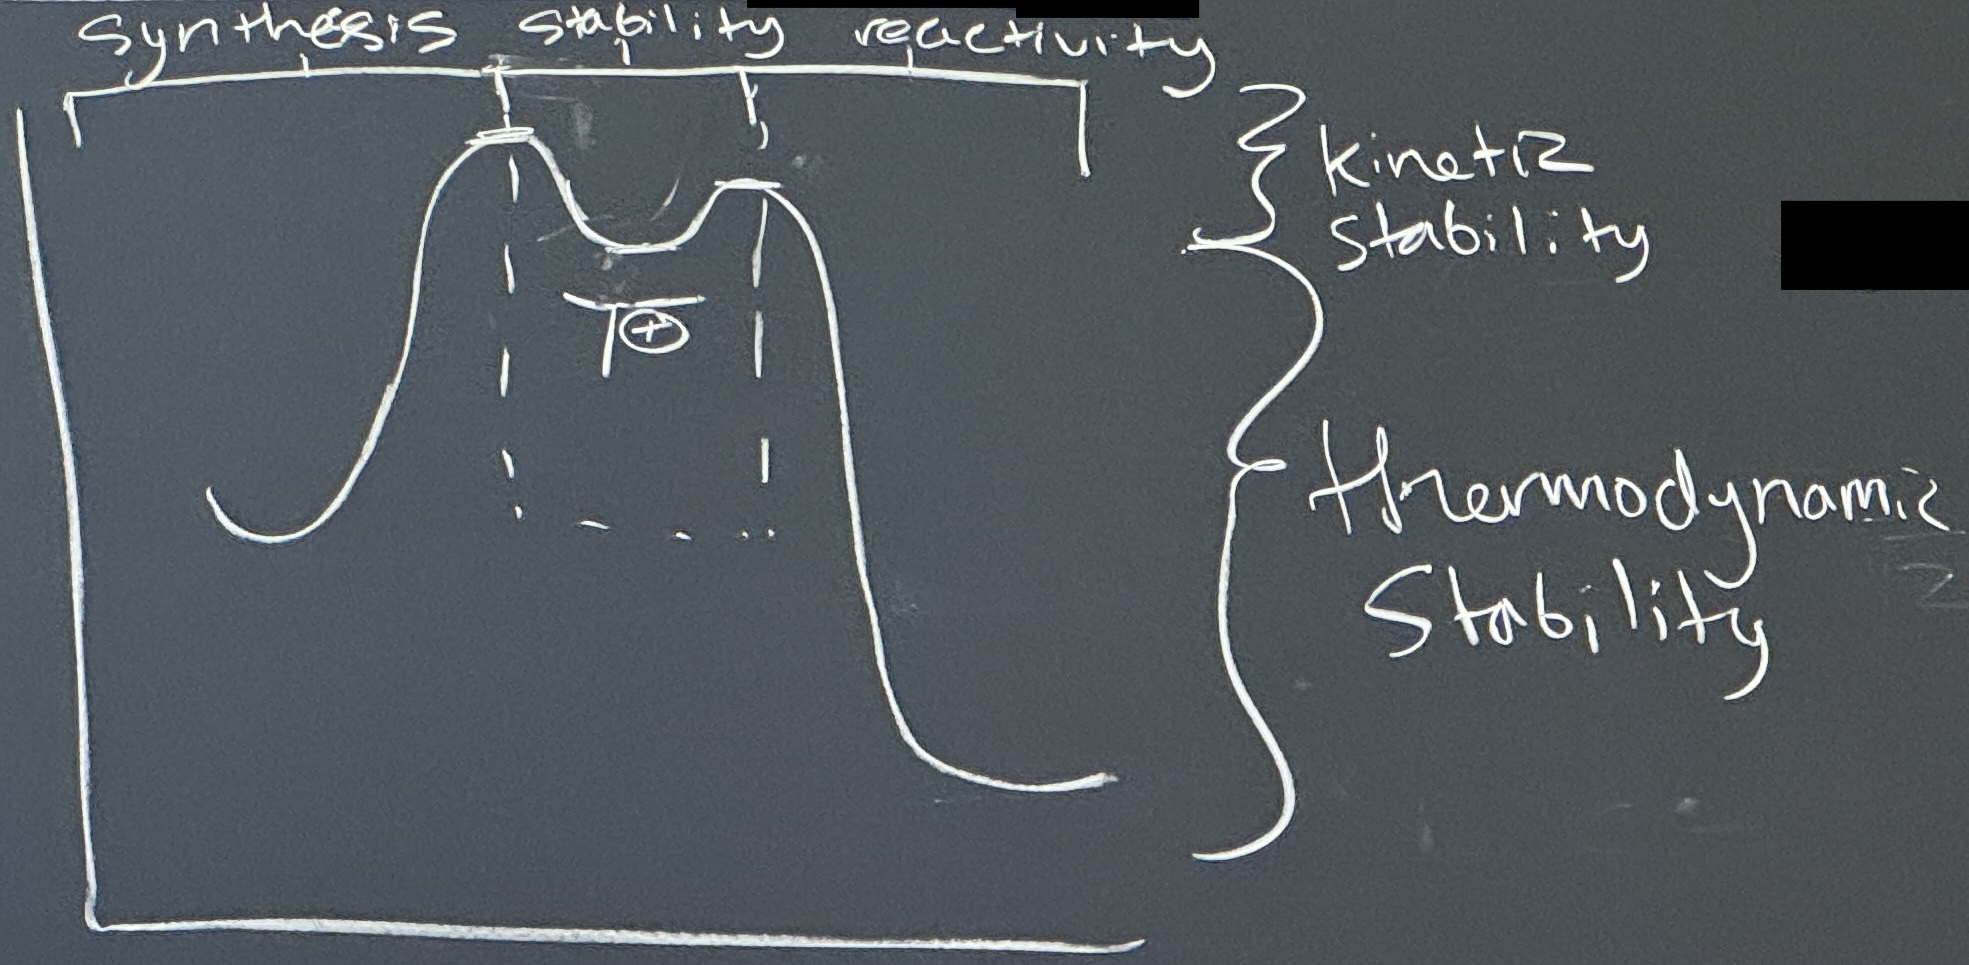
\includegraphics[width=0.5\linewidth]{catPhases.JPG}
        \caption{Phases in the life of a cation.}
        \label{fig:catPhases}
    \end{figure}
    \begin{itemize}
        \item All three phases correspond to specific regions along the reaction coordinate in the energy diagram for a cation-intermediate reaction.
        \item Stability, in particular, we'll talk about from a kinetic \emph{and} a thermodynamic perspective.
        \begin{itemize}
            \item Kinetic stability deals with the energy barrier to \emph{form} and to \emph{react} the cation.
            \item Thermodynamic stability deals with the energy difference between the cation and the adjacent local ground state structures.
        \end{itemize}
        \item Cations can have quite "sensitive" energy surfaces, i.e., factors that can stabilize and destabilize cations can have dramatic effects on the synthesis, stability, and reactivity of cations.
        \item Features that stabilize cations tend to lead to reactions.
        \begin{itemize}
            \item If you're in the lab, consider stabilizing the cation in order to induce the desired reactivity!
        \end{itemize}
    \end{itemize}
    \item Cation structure.
    \begin{figure}[h!]
        \centering
        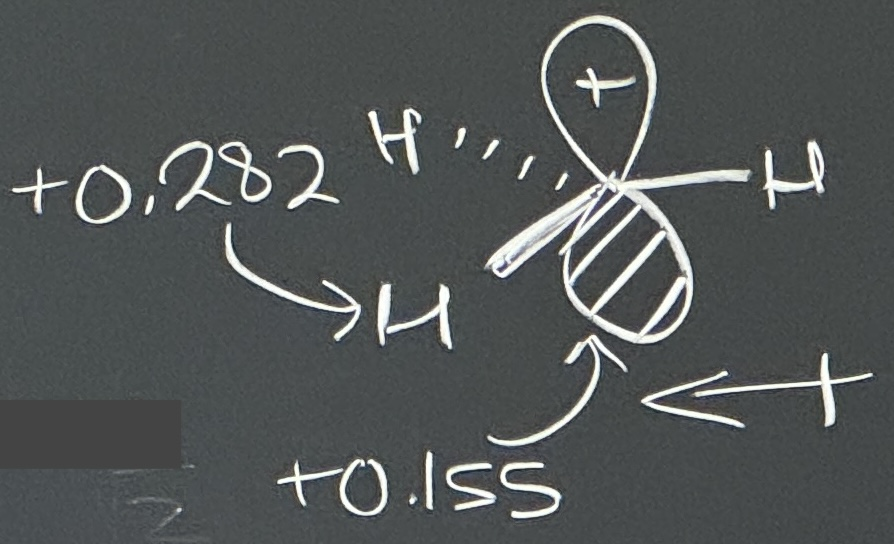
\includegraphics[width=0.2\linewidth]{structureCation.JPG}
        \caption{Cation structure.}
        \label{fig:structureCation}
    \end{figure}
    \begin{itemize}
        \item Figure \ref{fig:structureCation} depicts a methyl cation (\ce{{}^{$\oplus$}CH3}).
        \item In general, cations are $sp^2$-hybridized, trigonal planar species.
        \begin{itemize}
            \item Recall that Figure \ref{fig:QmotCH3} explains why cations are trigonal planar instead of pyramidal.
        \end{itemize}
        \item The cationic charge is delocalized across the entire molecule, not localized on the carbon.
        \begin{itemize}
            \item Indeed, there is a $\delta^+$ on the \ce{H}'s, too.
            \item In fact, the dipole qualitatively points \emph{toward} the carbon.
            \item Quantitatively, the \textbf{Mulliken partial charges} are $+0.155$ on \ce{C} and $+0.282$ on each \ce{H}. Together, these partial charges sum to the total charge of $+1$:
            \begin{equation*}
                1\times 0.155+3\times 0.282 \approx 1
            \end{equation*}
        \end{itemize}
    \end{itemize}
    \item Experimental evidence for cation formation.
    \begin{figure}[h!]
        \centering
        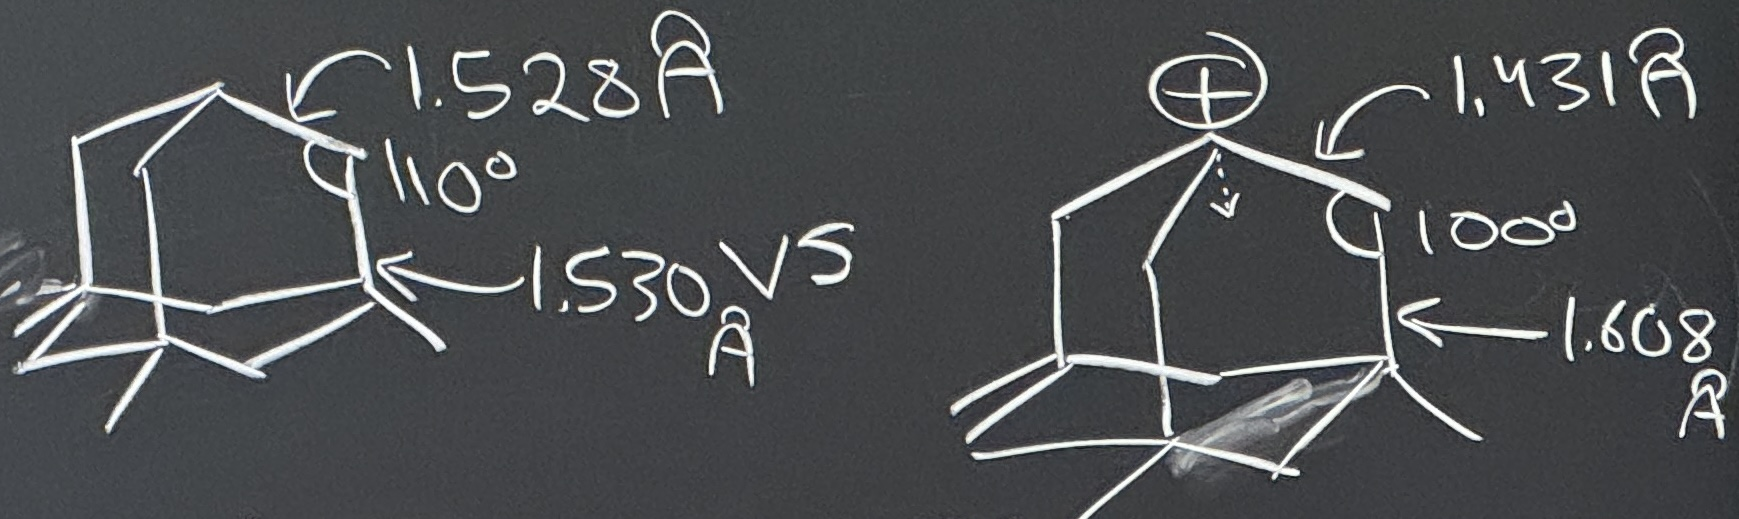
\includegraphics[width=0.43\linewidth]{catEvidence.JPG}
        \caption{Evidence that carbocations exist.}
        \label{fig:catEvidence}
    \end{figure}
    \begin{itemize}
        \item Experimental evidence primarily comes from some cool adamantane structures.
        \item For example, consider trimethyl adamantane and its corresponding cation. The cation has structural characteristics indicative of the "flattening" transformation we would expect. Specifically\dots
        \begin{itemize}
            \item The adjacent bond angles flatten from \ang{110} to \ang{100};
            \item The bonds immediately surrounding the cation shrink from \SI{1.528}{\angstrom} to \SI{1.431}{\angstrom} as the molecular geometry compresses the flattening cation;
            \item The bonds $\alpha,\beta$ to the cation elongate from \SI{1.530}{\angstrom} to \SI{1.608}{\angstrom} as electron density is removed from them through hyperconjugation and the no-bond resonance form.
        \end{itemize}
        \item Reference: \textcite{bib:catEvidence}.
    \end{itemize}
    \pagebreak
    \item Moving on, to measure the thermodynamic stability of a cation, we use the \textbf{hydride ion affinity}.
    \item \textbf{Hydride ion affinity}: The extent to which cations want to bind a hydride in solution. \emph{Also known as} \textbf{HIA}. \emph{Given by}
    \begin{equation*}
        \ce{RH <=> R+ + H-}\tag*{$\Delta H^\circ=\text{HIA}$}
    \end{equation*}
    \begin{itemize}
        \item Always measured in the gas phase.
        \item Only tells you the \emph{relative} stability.\footnote{Relative to what??}
    \end{itemize}
    \item Example HIAs.
    \begin{figure}[h!]
        \centering
        \footnotesize
        \setchemfig{atom sep=1.4em,arrow coeff=0.7}
        \setcharge{extra sep=5pt}
        \begin{subfigure}[b]{\linewidth}
            \centering
            \chemnameinit{\chemfig{*6(=-=(-)-=-)}}
            \schemestart
                \chemname{
                    \chemfig{-[:30]-[:-30]-[:30]\charge{0=$\oplus$}{}}
                }{266}
                \arrow(.base east--.base west){0}
                \chemname{
                    \chemfig{=_[:30]-[:-30]\charge{0=$\oplus$}{}}
                }{256}
                \arrow(.base east--.base west){0}
                \chemname{
                    \chemfig{*6(=-=(-\charge{0=$\oplus$}{})-=-)}
                }{239\hspace{1.7em}}
            \schemestop
            \chemnameinit{}
            \caption{The effect of resonance.}
            \label{fig:HIAexa}
        \end{subfigure}\\[2em]
        \begin{subfigure}[b]{0.68\linewidth}
            \centering
            \schemestart
                \chemname{
                    \chemfig{H_3\charge{0=$\oplus$}{C}}
                }{312}
                \arrow(.base east--.base west){0}
                \chemname{
                    \chemfig{-[:60](-[:120])-\charge{0=$\oplus$}{}}
                }{265}
                \arrow(.base east--.base west){0}
                \chemname{
                    \chemfig{-[:30]-[:-30]\charge{90=$\oplus$}{}-[:30]}
                }{247}
                \arrow(.base east--.base west){0}
                \chemname{
                    \chemfig{-[:60]\charge{60=$\oplus$}{}(-[:120])-}
                }{231}
                \arrow(.base east--.base west){0}
                \chemname{
                    \chemfig{-[:120]\charge{0=$\oplus$}{}(-[:60])-[4]*3(---)}
                }{218}
            \schemestop
            \chemnameinit{}
            \caption{The effect of hyperconjugation.}
            \label{fig:HIAexb}
        \end{subfigure}
        \begin{subfigure}[b]{0.3\linewidth}
            \centering
            \vspace{1.5em}
            \chemfig[atom sep=3em]{>[:160]@{C1}\charge{[extra sep=2.5em]90=$\oplus$}{}(<:[:20])-[4]@{C2}*3(-[@{1}]@{C3}-@{C4}-[@{2}])}
            \chemmove{
                \draw [thick,orx] ($(C1)+(0.0018,0.2)$) to[bend right=120,looseness=900] ($(C1)+(-0.0018,0.2)$) -- cycle;
                \filldraw [thick,draw=orx,fill=ory] ($(C1)+(0.0018,-0.2)$) to[bend left=120,looseness=900] ($(C1)+(-0.0018,-0.2)$) -- cycle;
                % 
                \draw [thick,orx,rotate=35] ($(C2)+(0.0018,0)$) to[bend right=130,looseness=700] ($(C2)+(-0.0018,0)$) -- cycle;
                \filldraw [thick,draw=orx,fill=ory,rotate=35] ($(C2)+(0.0018,0)$) to[bend left=130,looseness=200] ($(C2)+(-0.0018,0)$) -- cycle;
                \draw [thick,orx,rotate=-95] ($(C3)+(0.0018,0)$) to[bend right=130,looseness=700] ($(C3)+(-0.0018,0)$) -- cycle;
                \filldraw [thick,draw=orx,fill=ory,rotate=-95] ($(C3)+(0.0018,0)$) to[bend left=130,looseness=200] ($(C3)+(-0.0018,0)$) -- cycle;
                % 
                \filldraw [thick,draw=orx,fill=ory,rotate=95] ($(C4)+(0.0018,0)$) to[bend left=130,looseness=700] ($(C4)+(-0.0018,0)$) -- cycle;
                \draw [thick,orx,rotate=-95] ($(C4)+(0.0018,0)$) to[bend left=130,looseness=200] ($(C4)+(-0.0018,0)$) -- cycle;
                \filldraw [thick,draw=orx,fill=ory,rotate=-35] ($(C2)+(0.0018,0)$) to[bend left=130,looseness=700] ($(C2)+(-0.0018,0)$) -- cycle;
                \draw [thick,orx,rotate=-35] ($(C2)+(0.0018,0)$) to[bend right=130,looseness=200] ($(C2)+(-0.0018,0)$) -- cycle;
                % 
                \draw [thick,orx,rotate=-25] ($(C3)+(0.0018,0)$) to[bend left=130,looseness=700] ($(C3)+(-0.0018,0)$) -- cycle;
                \filldraw [thick,draw=orx,fill=ory,rotate=-25] ($(C3)+(0.0018,0)$) to[bend right=130,looseness=200] ($(C3)+(-0.0018,0)$) -- cycle;
                \draw [thick,orx,rotate=25] ($(C4)+(0.0018,0)$) to[bend right=130,looseness=700] ($(C4)+(-0.0018,0)$) -- cycle;
                \filldraw [thick,draw=orx,fill=ory,rotate=25] ($(C4)+(0.0018,0)$) to[bend left=130,looseness=200] ($(C4)+(-0.0018,0)$) -- cycle;
                % 
                \draw [curved arrow={1.3em}{1em}] (1) to[out=60,in=150,looseness=1.3] ([yshift=2em]C1.center);
                \draw [curved arrow={1.3em}{1em}] (2) to[out=-60,in=-150,looseness=1.3] ([yshift=-2em]C1.center);
            }
            \vspace{2.3em}
            \caption{Cyclopropyl stabilization.}
            \label{fig:HIAexc}
        \end{subfigure}\\[2em]
        \begin{subfigure}[b]{0.98\linewidth}
            \centering
            \chemnameinit{\chemfig{H_2N-[:30]}}
            \schemestart
                \chemname{
                    \chemfig{-[:30]\charge{0=$\oplus$}{}}
                }{273}
                \arrow(.base east--.base west){0}
                \chemname{
                    \chemfig{HO-[:30]\charge{0=$\oplus$}{}}
                }{243}
                \arrow(.base east--.base west){0}
                \chemname{
                    \chemfig{H_2N-[:30]\charge{0=$\oplus$}{}}
                }{218}
            \schemestop
            \caption{The effect of heteroatoms.}
            \label{fig:HIAexd}
        \end{subfigure}
        \chemnameinit{}
        \caption{Hydride ion affinity examples.}
        \label{fig:HIAex}
    \end{figure}
    \begin{itemize}
        \item Alkyl, allylic, and benzylic HIAs (Figure \ref{fig:HIAexa}).
        \begin{itemize}
            \item Respectively: \SI[per-mode=symbol]{266}{\kilo\calorie\per\mole}, \SI[per-mode=symbol]{256}{\kilo\calorie\per\mole}, and \SI[per-mode=symbol]{239}{\kilo\calorie\per\mole}.
            \item Attributable to resonance delocalization and conjugation.
        \end{itemize}
        \item Methyl, isobutyl, \emph{sec}-butyl, \emph{tert}-butyl, and dimethylcyclopropyl HIAs (Figure \ref{fig:HIAexb}).
        \begin{itemize}
            \item Respectively: \SI[per-mode=symbol]{312}{\kilo\calorie\per\mole}, \SI[per-mode=symbol]{265}{\kilo\calorie\per\mole}, \SI[per-mode=symbol]{247}{\kilo\calorie\per\mole}, \SI[per-mode=symbol]{231}{\kilo\calorie\per\mole}, and \SI[per-mode=symbol]{218}{\kilo\calorie\per\mole}.
            \item Attributable to hyperconjugation.
            \item Deeper dive: Hyperconjugation from cyclopropyl rings (Figure \ref{fig:HIAexc})
            \begin{itemize}
                \item This is a follow up to our brief discussion on the same topic in Lecture 3.
                \item When this molecule forms, the carbocation's empty $p$-orbital will align with the $\sigma$-plane of the cyclopropyl group.
                \item With this alignment, \emph{both} adjacent \ce{C-C} banana bonds can donate into the carbocation through hyperconjugation.
                \item The hyperconjugative interaction is so extreme that the barrier to rotation along the bond between the cation and the cyclopropyl group is \SI{13.7}{kcal/mol}!
                \item We can also picture this interaction through no-bond resonance forms that delocalize the positive charge to the back two carbons in the cyclopropyl group.
                \item You can look up the crystal structure of this molecule to see the interaction more.
            \end{itemize}
        \end{itemize}
        \item Ethyl, hydroxymethyl, and aminomethyl HIAs (Figure \ref{fig:HIAexd}).
        \begin{itemize}
            \item Respectively: \SI[per-mode=symbol]{273}{\kilo\calorie\per\mole}, \SI[per-mode=symbol]{243}{\kilo\calorie\per\mole}, and \SI[per-mode=symbol]{218}{\kilo\calorie\per\mole}.
            \item Attributable to heteroatom stabilization (aka resonance).
        \end{itemize}
    \end{itemize}
    \pagebreak
    \item The stability of the carbocation (as discussed above in terms of HIAs) determines how high the local minimum is in the energy diagram in Figure \ref{fig:catPhases}.
    \item We now move onto the kinetic stability/reactivity of cations.
    \item Two ways of measuring this.
    \begin{enumerate}
        \item Rates of \textbf{solvolysis}.
        \begin{itemize}
            \item Used all the time.
        \end{itemize}
        \item \textbf{Mayr electrophilicity}.
        \begin{itemize}
            \item More niche, but still good to know.
        \end{itemize}
    \end{enumerate}
    \item \textbf{Solvolysis}: A type of nucleophilic substitution (S\textsubscript{N}1 or S\textsubscript{N}2) wherein the nucleophile is a solvent molecule. \emph{Given by}
    \begin{equation*}
        \ce{R3C-X + H2O ->[$k_\text{rel}$][\Delta] R3C-OH + XH}
    \end{equation*}
    \begin{itemize}
        \item Rates of solvolysis are reported as a relative rate constant $k_\text{rel}$.
    \end{itemize}
    \item Comparing HIAs to rates of solvolysis.
    \begin{table}[h!]
        \centering
        \small
        \renewcommand{\arraystretch}{1.2}
        \begin{tabular}{l|ccc}
             & \textbf{\ce{Bn-Br}} & \textbf{\ce{All-Br}} & \textbf{\ce{{}^{\emph{i}}Pr-Br}}\\
            \hline
            \textbf{HIA (\ce{R+})} & 239 & 256 & 249\\
            $\bm{k_\textbf{rel}}$ & 100 & 52 & 0.7\\
        \end{tabular}
        \caption{HIAs and the rate of solvolysis are not correlated.}
        \label{tab:HIAk}
    \end{table}
    \begin{itemize}
        \item To be clear, we are listing the HIA of the benzyl, allyl, and isopropyl cations.
        \item Benzyl bromide affords a cation that is both the most stable and the most reactive in the set.\footnote{Clarify??}
        \item Note that in general, solution-phase measures of stability like solvolysis and gas-phase measures of stability like the HIA \emph{don't} correlate. This means that we do have to measure them independently.
    \end{itemize}
    \item \textbf{Mayr electrophilicity}: The rate of reaction for various electrophilic and nucleophile pairs. \emph{Given by}
    \begin{equation*}
        \ce{E+ + Nuc- ->[$k$] Nuc-E}
    \end{equation*}
    \begin{itemize}
        \item By Herbert Mayr from 5.47!
        \item Mayr defined three parameters ($S$, $N$, and $E$) via the equation.
        \begin{equation*}
            \log k = s(N+E)
        \end{equation*}
        \begin{itemize}
            \item $s$ is a nucleophile-specific slope parameter.
            \item $N$ is a nucleophile parameter.
            \item $E$ is an electrophile parameter.
        \end{itemize}
        \item Note that "\ce{Nuc-}" indicates a nucleophile, just like the more commonly used \ce{Nu-}.
        \item Mayr has done hundreds of these reactions, measured their rates, had reference nucleophile, etc.
        \begin{itemize}
            \item His group is still expanding the chart!
            \item There's a giant PDF on Mayr's \href{https://www.cup.uni-muenchen.de/oc/mayr/DBintro.html}{website} that we can download if we want.
        \end{itemize}
        \item Reference: \textcite{bib:Mayr}.
    \end{itemize}
    \pagebreak
    \item Example Mayr electrophilicities.
    \begin{figure}[h!]
        \centering
        \footnotesize
        \setchemfig{atom sep=1.4em}
        \setcharge{extra sep=5pt}
        \schemestart
            \chemname{
                \chemfig{Ph-[:30]\charge{30=$\oplus$}{}(-[2])-[:-30]}
            }{$5.7$}
            \arrow(.base east--.base west){0}
            \chemname{\subscheme{
                \chemfig{Ph-[:30]\charge{90=$\oplus$}{}(-[2,0.6,,,opacity=0])-[:-30]OMe}
                \arrow{<->}[90,0.8]
                \chemfig{Ph-[:30]=_[:-30]\charge{90=$\oplus$}{O}Me}
            }}{$3.0$}
            \arrow(.base east--.base west){0}
            \chemname{\subscheme{
                \chemfig{-[:60]N(-[:120])-\charge{0=$\oplus$}{}}
                \arrow{<->}[90,0.8]
                \chemfig{-[:60]\charge{60=$\oplus$}{N}(-[:120])=}
            }}{$-6.5$}
        \schemestop
        \chemnameinit{}
        \caption{Mayr electrophilicity examples.}
        \label{fig:Mayr}
    \end{figure}
    \begin{itemize}
        \item To be clear, Figure \ref{fig:Mayr} lists the $E$ value for each species.
        \item Remember that Mayr electrophilicity is reported on a logarithmic scale, so the difference in $E$ between the left two species (approximately 3) corresponds to a difference in reactivity of three \emph{orders of magnitude}.
        \begin{itemize}
            \item Similarly, the difference in reactivity between the right two species is \emph{nine orders of magnitude}!
        \end{itemize}
        \item Some of these trends should make sense.
        \begin{itemize}
            \item For example, it stands to reason that the cation with heteroatom stabilization is the least electrophilic.
        \end{itemize}
        \item Observe that our most thermodynamically stable carbocation (the $3^\circ$ one with extensive resonance into the phenyl ring) is also our most Mayr electrophilic one!
        \begin{itemize}
            \item This is yet another example of thermodynamics being decoupled from the kinetics of reactivity.
        \end{itemize}
    \end{itemize}
    \item This concludes our discussion of \emph{measuring} kinetic and thermodynamic stability. Let's now talk about \emph{enhancing} carbocation stability.
    \item Four ways of doing this.
    \begin{enumerate}
        \item \textbf{Hyperconjugation}.
        \item Heteroatom stabilization.
        \item The \textbf{$\bm{\beta}$-silicon effect}.
        \item The \textbf{neighboring group effect}.
    \end{enumerate}
    \item \textbf{Hyperconjugation}: The delocalization of electrons through $\sigma$-bonds.
    \begin{figure}[h!]
        \centering
        \begin{subfigure}[b]{0.3\linewidth}
            \centering
            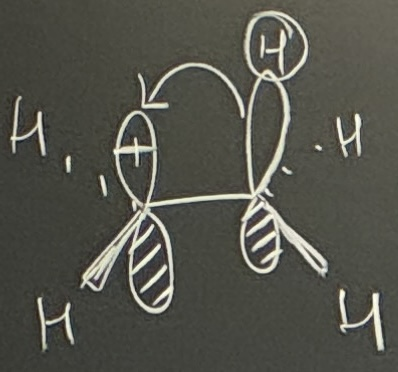
\includegraphics[width=0.37\linewidth]{hyperconjugationa.JPG}
            \caption{$\sigma_{\ce{CH}}\to p_{\ce{C}}$ donation.}
            \label{fig:hyperconjugationa}
        \end{subfigure}
        \begin{subfigure}[b]{0.3\linewidth}
            \centering
            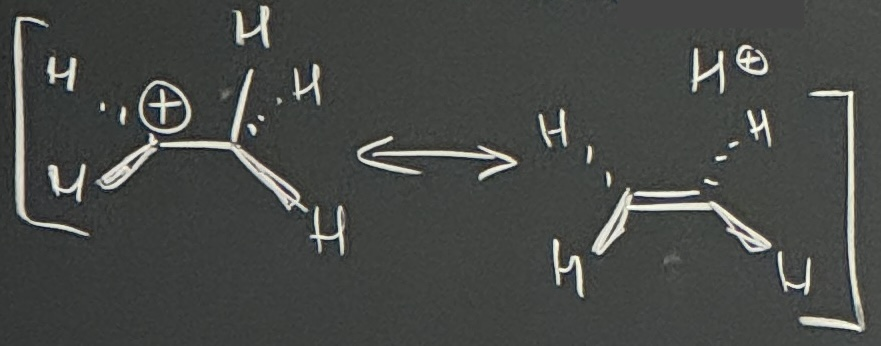
\includegraphics[width=0.9\linewidth]{hyperconjugationb.JPG}
            \caption{No-bond resonance.}
            \label{fig:hyperconjugationb}
        \end{subfigure}
        \caption{Stabilizing carbocations: Hyperconjugation.}
        \label{fig:hyperconjugation}
    \end{figure}
    \begin{itemize}
        \item Hyperconjugation explains why substituted cations are more stable.
        \item Recall from 5.13\footnote{Figure \ref{fig:hyperconjugationa} is just Figure 2.3a from \textcite{bib:5-13Notes}.} that the ethyl cation is stabilized by $\sigma_{\ce{CH}}\to p_{\ce{C}}$ donation.
        \item Equivalently, we can say that the ethyl cation is stabilized by \textbf{no-bond resonance}.
        \begin{itemize}
            \item What this really tells us is that the \ce{C-C} bond is shorter than we'd normally expect, and the \ce{C-H} bond is longer than we'd normally expect.
        \end{itemize}
    \end{itemize}
    \pagebreak
    \item Example HIA differences caused by hyperconjugation (Figure \ref{fig:HIAexb}).
    \begin{itemize}
        \item Increasing from no adjacent \ce{C-C} bonds to three adjacent \ce{C-C} bonds decreases the HIA from \SI[per-mode=symbol]{312}{\kilo\calorie\per\mole} to \SI[per-mode=symbol]{231}{\kilo\calorie\per\mole}.
        \item Essentially, as we add more \ce{R} groups, the cation's empty $p$-orbital gets stabilized by additional adjacent $\sigma$-orbitals.
    \end{itemize}
    \item Matthew: Does hyperconjugation induce a barrier to rotation?
    \begin{itemize}
        \item There's always some barrier.
        \begin{itemize}
            \item In a normal alkyl molecule, it's approx \SI[per-mode=symbol]{3}{\kilo\calorie\per\mole}.
        \end{itemize}
        \item In a hyperconjugated cation, we will see bigger differences.
        \begin{itemize}
            \item In fact, there's a fascinating example somewhere in the literature of the stereochemistry of a product being determined by geometric constraints caused by hyperconjugation!
        \end{itemize}
        \item So all this is to say, yes.
    \end{itemize}
    \item Heteroatom stabilization.
    \begin{figure}[h!]
        \centering
        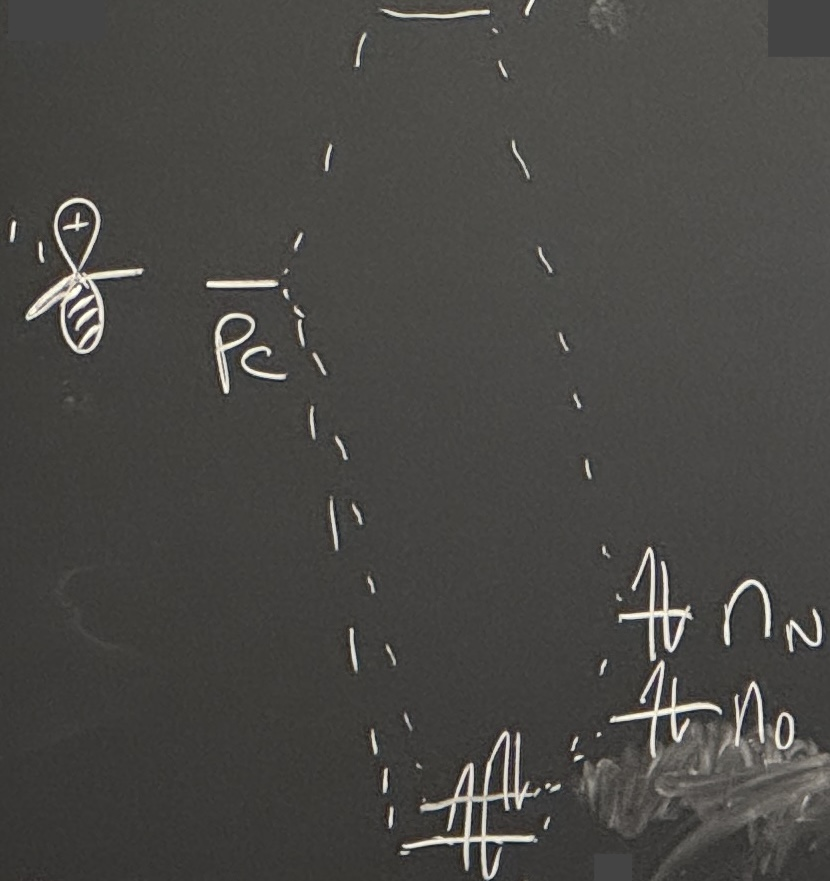
\includegraphics[width=0.2\linewidth]{heteroatomCC.JPG}
        \caption{Stabilizing carbocations: Adjacent heteroatoms.}
        \label{fig:heteroatomCC}
    \end{figure}
    \begin{itemize}
        \item The high-energy empty $p$-orbital on carbon and low-energy heteroatom lone pair interact to form new bonding and antibonding MOs.
        \begin{itemize}
            \item The bonding MO will be lower energy than the lone pair AO, so the electrons in that lone pair will be stabilized.
        \end{itemize}
        \item Nitrogen vs. oxygen stabilization: Rationalizing why nitrogen is more stabilizing in Figure \ref{fig:HIAexd}.
        \begin{itemize}
            \item The $n_{\ce{O}}$ AO is lower in energy than the $n_{\ce{N}}$ AO.
            \item This means that there is worse energy overlap between the $n_{\ce{O}}$ AO and the $p_{\ce{C}}$ AO than between the $n_{\ce{N}}$ AO and the $p_{\ce{C}}$ AO.
            \item The worse energy overlap with oxygen leads to a resultant decrease in MO splitting, and hence less stabilization for the oxygen lone pair than the nitrogen lone pair receives.
        \end{itemize}
    \end{itemize}
    \item \textbf{$\bm{\beta}$-silicon effect}: The stabilization of positive charge at the position $\beta$ to a silicon atom.
    \begin{itemize}
        \item Caused by hyperconjugation.
        \item Specifically, silicon is a better $\sigma$-donor, by which we mean that \ce{C-Si} bonds are better at sharing their electron density via hyperconjugation than \ce{C-C} or \ce{C-H} bonds.\footnote{Note that we do \emph{not} mean that silicon is a better $\sigma$-donor ligand, like in inorganic chemistry.}
        \item Silicon is better because\dots
        \begin{itemize}
            \item Silicon is less electronegative than other common $\sigma$-donors;
            \begin{itemize}
                \item Indeed, $\text{EN}_{\ce{C}}=2.55$ and $\text{EN}_{\ce{C}}=2.20$, but $\text{EN}_{\ce{Si}}=1.90$.
                \item Thus, \ce{C-Si} bonds hold their electrons less tightly and hence are happier to share.
                \item \ce{C-Si} bonds holding their electrons less tightly also implies the following.
            \end{itemize}
            \item \ce{C-Si} bonds are longer;
            \begin{itemize}
                \item \SI{1.86}{\angstrom} vs. the \SI{1.54}{\angstrom} typical of a \ce{C-C} bond.
                \item This allows for greater overlap with the typically lengthy $p$-orbitals.
            \end{itemize}
            \item \ce{C-Si} bonds are more ionic;
            \begin{itemize}
                \item Polarization toward carbon (more ionicness) means that there's more electron density on the carbon (i.e., near the carbocation).
            \end{itemize}
            \item The $\sigma_{\ce{CSi}}$ orbital is higher in energy than $\sigma_{\ce{CC}}$ orbital.
            \begin{itemize}
                \item Thus, like in Figure \ref{fig:heteroatomCC}, we get closer to the $p_{\ce{C}}$ energy level and have more effective overlap.
            \end{itemize}
        \end{itemize}
    \end{itemize}
    \item Example HIA differences caused by the $\beta$-silicon effect.
    \begin{figure}[h!]
        \centering
        \begin{subfigure}[b]{0.25\linewidth}
            \centering
            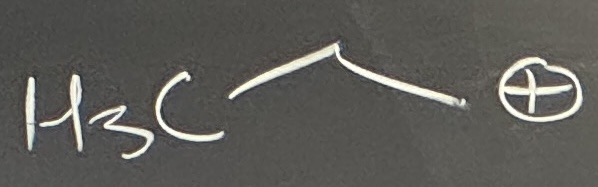
\includegraphics[width=0.45\linewidth]{HIAbSia.JPG}
            \caption{$\text{HIA}=\SI[per-mode=symbol]{266}{\kilo\calorie\per\mole}$.}
            \label{fig:HIAbSia}
        \end{subfigure}
        \begin{subfigure}[b]{0.25\linewidth}
            \centering
            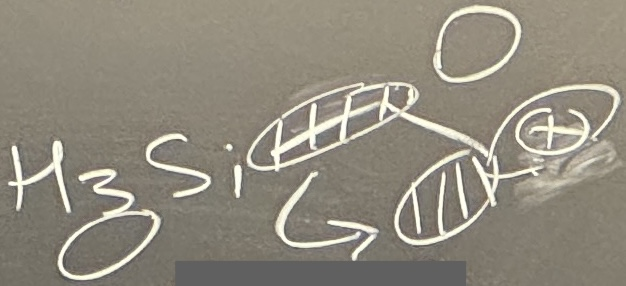
\includegraphics[width=0.55\linewidth]{HIAbSib.JPG}
            \caption{$\text{HIA}=\SI[per-mode=symbol]{228}{\kilo\calorie\per\mole}$.}
            \label{fig:HIAbSib}
        \end{subfigure}
        \caption{Hydride ion affinities subject to the $\beta$-silicon effect.}
        \label{fig:HIAbSi}
    \end{figure}
    \begin{itemize}
        \item Changing an alkyl cation to the direct silicon analogue alters the HIA by nearly \SI[per-mode=symbol]{40}{\kilo\calorie\per\mole}.
    \end{itemize}
    \item Examples of how the $\beta$-silicon effect alters reactivity.
    \begin{figure}[h!]
        \centering
        \begin{subfigure}[b]{\linewidth}
            \centering
            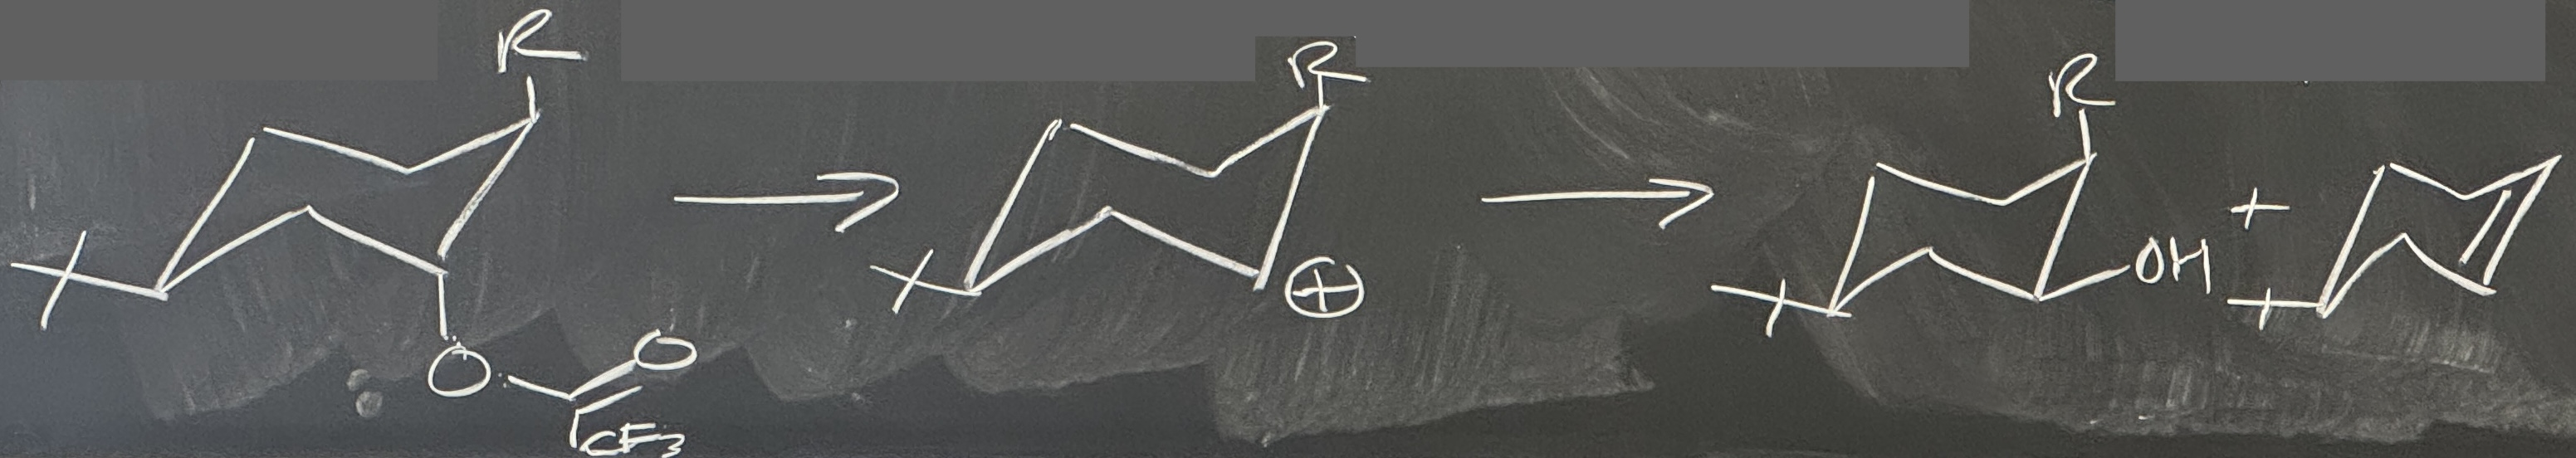
\includegraphics[width=0.7\linewidth]{bSiReacta.JPG}
            \caption{Accelerating S\textsubscript{N}1 and E\textsubscript{1}.}
            \label{fig:bSiReacta}
        \end{subfigure}\\[2em]
        \begin{subfigure}[b]{\linewidth}
            \centering
            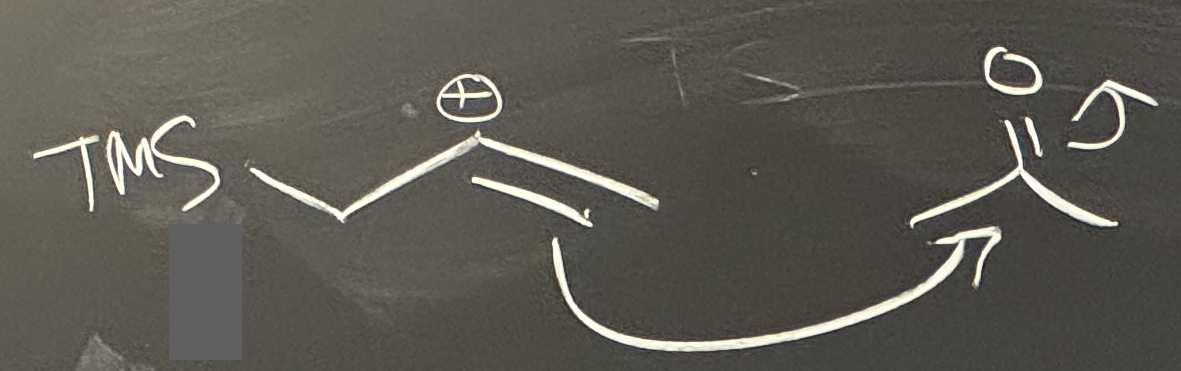
\includegraphics[width=0.25\linewidth]{bSiReactb.JPG}
            \caption{Enabling allylations.}
            \label{fig:bSiReactb}
        \end{subfigure}
        \caption{The $\beta$-silicon effect enables cationic reactivity.}
        \label{fig:bSiReact}
    \end{figure}
    \begin{itemize}
        \item It can accelerate the departure of a leaving group by orders of magnitude (Figure \ref{fig:bSiReacta}).
        \begin{itemize}
            \item Suppose we have a trifluoroacetate leaving group on a cyclohexane ring in aqueous solution.
            \item Locking \ce{F3CCO2-} in the axial position with an equatorial \emph{tert}-butyl group aids departure.
            \begin{itemize}
                \item Specifically, if $\ce{R}=\ce{SiMe3}$, the anomeric effect will significantly weaken the \ce{C-O} bond.
            \end{itemize}
            \item Once \ce{F3CCO2-} leaves, the reaction completes through hydration (S\textsubscript{N}1) or elimination (E\textsubscript{1}).
            \item If $k_\text{rel}=1$ when $\ce{R}=\ce{H}$, then $k_\text{rel}=\num{2.4e12}$ when $\ce{R}=\ce{SiMe3}$.
            \begin{itemize}
                \item There's a reason this effect has a name: It's huge!
            \end{itemize}
        \end{itemize}
        \item It enables allylations to happen at all (Figure \ref{fig:bSiReactb}).
        \begin{itemize}
            \item We do allylations with allyl silane because it's the only way this will work.
            \item The allyl group attacks the carbonyl as a nucleophile, forming a secondary carbocation that's stabilized by the $\beta$-silicon effect at the indicated position.
            \item Note that this reaction is \emph{not} an already-formed carbocation somehow engaging in a nucleophilic attack, despite how it's drawn. Here's a helpful \href{https://www.uwindsor.ca/people/jgreen/sites/uwindsor.ca.people.jgreen/files/41-45.pdf}{reference} on this type of reactivity.
        \end{itemize}
    \end{itemize}
    \item Motivating the neighboring group effect.
    \begin{figure}[H]
        \centering
        \begin{subfigure}[b]{\linewidth}
            \centering
            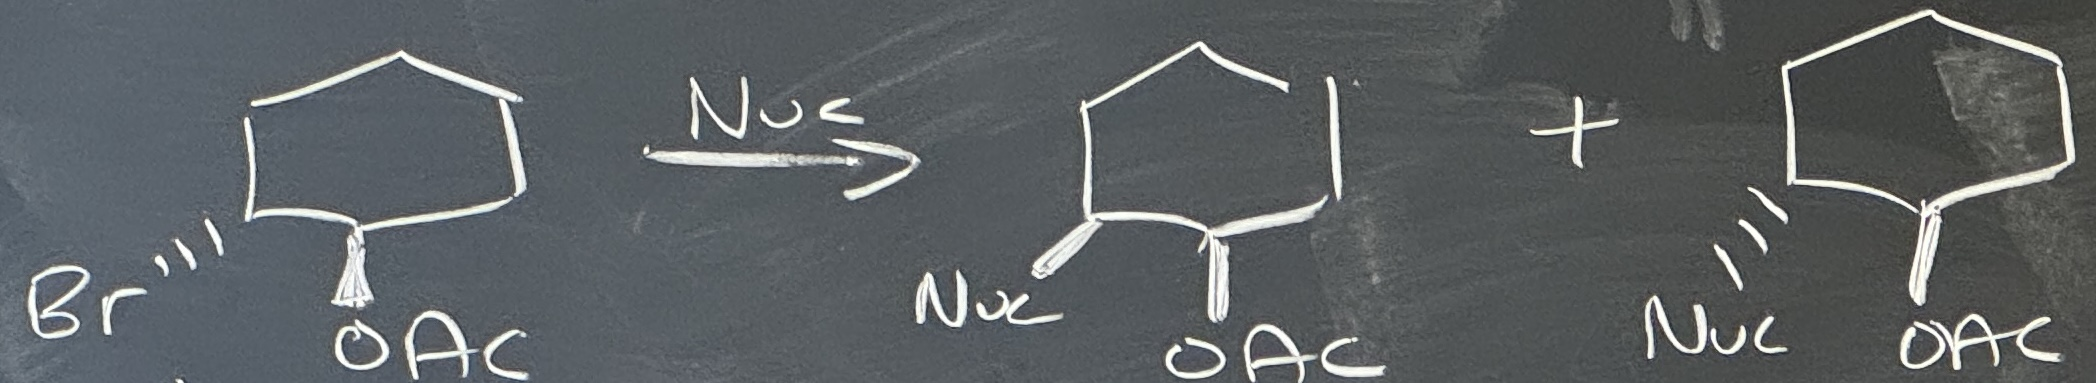
\includegraphics[width=0.5\linewidth]{neighbora.JPG}
            \caption{The possible products of a reaction.}
            \label{fig:neighbora}
        \end{subfigure}\\[2em]
        \begin{subfigure}[b]{\linewidth}
            \centering
            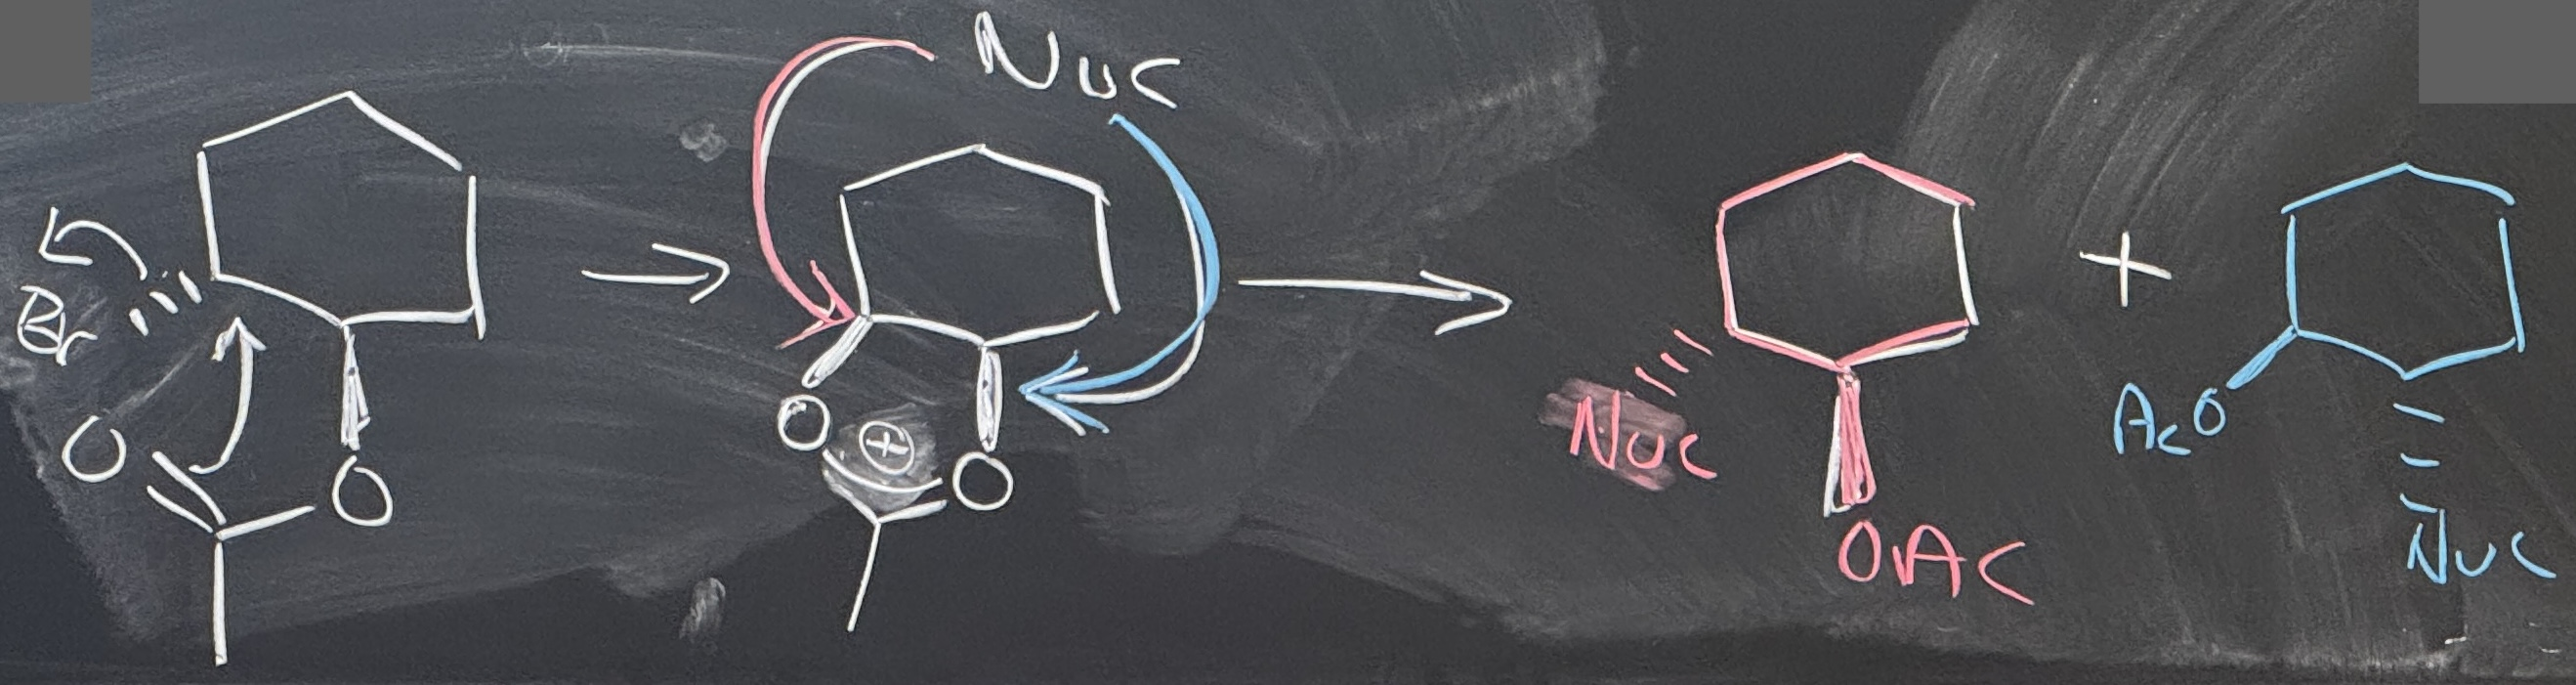
\includegraphics[width=0.6\linewidth]{neighborb.JPG}
            \caption{The mechanism of the reaction.}
            \label{fig:neighborb}
        \end{subfigure}
        \caption{The neighboring group effect alters cationic reactivity.}
        \label{fig:neighbor}
    \end{figure}
    \begin{itemize}
        \item The reaction in Figure \ref{fig:neighbora} is a nucleophilic substitution with an enantiopure starting material, and it has four possible product stereoisomers.
        \item Through which mechanisms could this reaction proceed?
        \begin{itemize}
            \item If S\textsubscript{N}2: We'll see 100\% \emph{syn} and 0\% \emph{anti} product because S\textsubscript{N}2 is stereospecific.
            \begin{itemize}
                \item The syn product will be enantiopure due to the stereoinverting nature of the attack.
            \end{itemize}
            \item If S\textsubscript{N}1: We'll see 50\% \emph{syn} and 50\% \emph{anti}, maybe favoring \emph{anti} a bit due to sterics.
            \begin{itemize}
                \item Both diastereomers will be enantipure (we're not engaging the acetate's chiral carbon).
            \end{itemize}
            \item Observed: We get 0\% \emph{syn} and 100\% \emph{anti}, and it's a racemic mixture of the \emph{anti} diastereomer.
        \end{itemize}
        \item What's happening here?!
        \begin{itemize}
            \item The acyl group is not as innocent as it seems.
            \item Per Figure \ref{fig:neighborb}, the actual mechanism begins with intramolecular displacement of the bromine to form a resonance-stabilized carbocation. This is followed by a backside attack on \emph{either} carbon, hence selecting the \emph{anti} product and inducing the racemization.
            \item Conclusion: The neighboring group effect makes this reaction \emph{trans}-selective and racemizing.
        \end{itemize}
    \end{itemize}
    \item \textbf{Neighboring group effect}: The interaction of a reaction center with either an intramolecular lone pair or an intramolecular pair of $\pi$-electrons. \emph{Also known as} \textbf{anchimeric assistance}.
    \begin{itemize}
        \item Note that the intramolecular pair of $\pi$-electrons cannot be conjugated with the reaction center; that's just resonance stabilization of the carbocation then.
    \end{itemize}
    \item \textbf{Homoconjugation}: A neighboring group effect in which the neighboring group is a $\pi$-system.\footnote{This definition is consistent with the definition of homoconjugation as "an overlap of two $\pi$-systems separated by a non-conjugating group" because the carbocation counts as a $\pi$-system and the carbocation in Figure \ref{fig:homoconjugation} is separated from the $\pi$-bond by one methylene group on each side.}
    \item Example of homoconjugation.
    \begin{figure}[H]
        \centering
        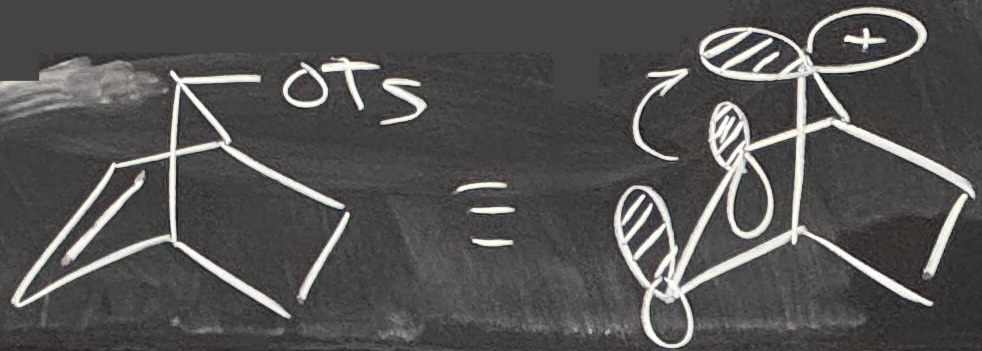
\includegraphics[width=0.25\linewidth]{homoconjugation.JPG}
        \caption{Homoconjugation.}
        \label{fig:homoconjugation}
    \end{figure}
    \begin{itemize}
        \item Essentially, the displacement of the tosyl group in Figure \ref{fig:homoconjugation} is much more favorable in the molecule shown than in the saturated analog because a double bond is present nearby (in the unsaturated molecule), and its $\pi$-orbitals can donate into the carbocation.
        \item Something like 5 orders of magnitude faster.\footnote{Actually 11 orders of magnitude per \href{https://en.wikipedia.org/wiki/Neighbouring_group_participation\#NGP_by_an_alkene}{Wikipedia}.}
    \end{itemize}
    \item We're now done with carbocation stability, and we'll begin discussing their synthesis and reactivity.
    \item Acidity.
    \begin{figure}[h!]
        \centering
        \footnotesize
        \schemestart
            \chemfig{Ph-[:30]\charge{[extra sep=5pt]90=$\oplus$}{}-[:-30]-[:30]H}
            \arrow
            \chemfig{Ph-[:30]=_[:-30]}
        \schemestop
        \caption{Carbocations acidify $\beta$-protons.}
        \label{fig:ccAcidify}
    \end{figure}
    \begin{itemize}
        \item Carbocations induce a dramatic acidification of $\beta$ \ce{C-H} bonds.
        \item Indeed, the $\pKa$ of the proton drawn in Figure \ref{fig:ccAcidify} is $-14$!
        \item Additionally, this reaction is just the second step in an E\textsubscript{1} mechanism: Adjacent deprotonation is just elimination!
        \begin{itemize}
            \item The reaction is purely downhill thermodynamically, and adjacent deprotonation is actually a great perspective to take on E\textsubscript{1}.
        \end{itemize}
    \end{itemize}
    \item Synthesis of carbocations: Two main ways.
    \begin{figure}[h!]
        \centering
        \footnotesize
        \begin{subfigure}[b]{0.4\linewidth}
            \centering
            \schemestart
                \chemfig{-[:60](-[:120])-(-[:-60]LG)-[:60]}
                \arrow
                \chemfig{-[:60](-[:120])-\charge{[extra sep=5pt]-60=$\oplus$}{}-[:60]}
            \schemestop
            \caption{Ionization.}
            \label{fig:ccSynthesisa}
        \end{subfigure}
        \begin{subfigure}[b]{0.4\linewidth}
            \centering
            \schemestart
                \chemfig{-[:60](-[:120])-=^[:60]}
                \arrow{->[\ce{E+}]}
                \chemfig{-[:60](-[:120])-\charge{[extra sep=5pt]-60=$\oplus$}{}-[:60]-E}
            \schemestop
            \caption{$\pi$-activation.}
            \label{fig:ccSynthesisb}
        \end{subfigure}
        \caption{Synthesis of carbocations.}
        \label{fig:ccSynthesis}
    \end{figure}
    \begin{enumerate}
        \item Ionization.
        \begin{itemize}
            \item This is just the departure of a leaving group.
        \end{itemize}
        \item Activation of a $\pi$-system.
        \begin{itemize}
            \item Can be done by an electrophile, such as a proton, metal, etc.
            \item Gives the Markovnikov adduct.
        \end{itemize}
    \end{enumerate}
    \item Reactions of cations.
    \begin{figure}[H]
        \centering
        \begin{subfigure}[b]{\linewidth}
            \centering
            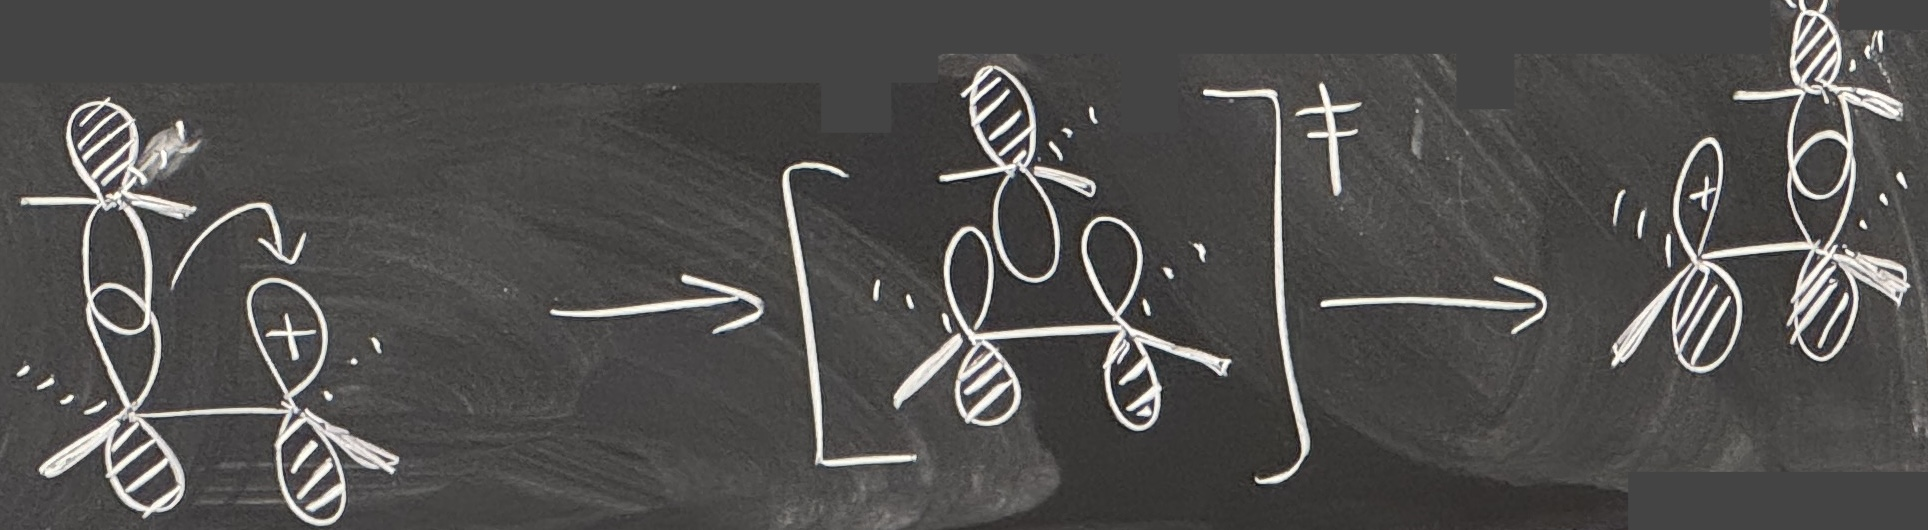
\includegraphics[width=0.45\linewidth]{ccReactiona.JPG}
            \caption{$[1,2]$-sigmatropic shift.}
            \label{fig:ccReactiona}
        \end{subfigure}\\[2em]
        \begin{subfigure}[b]{\linewidth}
            \centering
            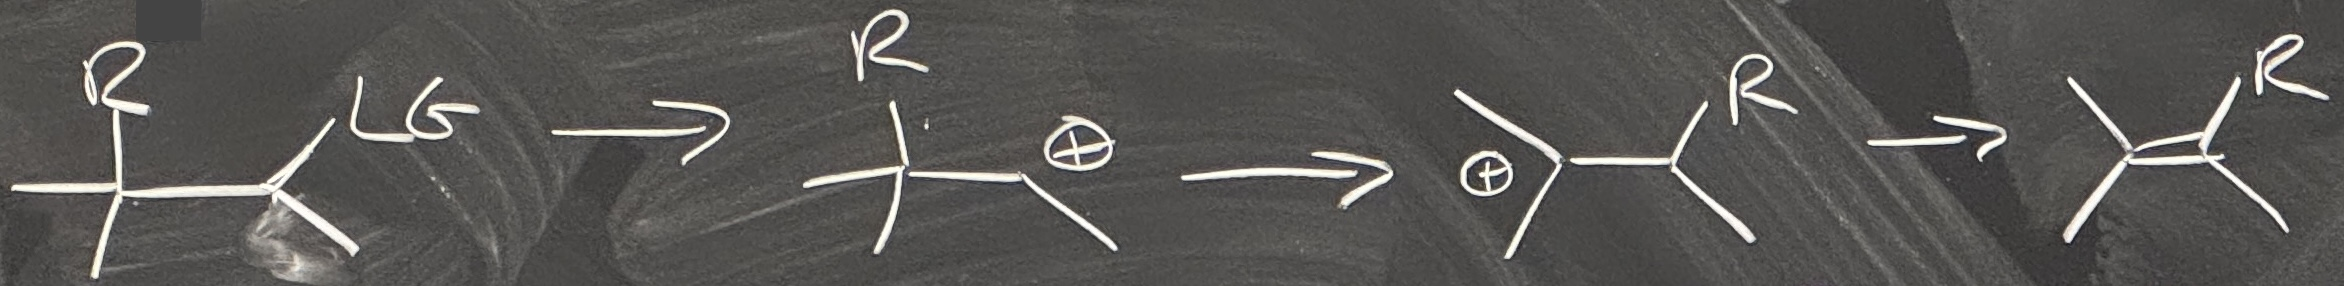
\includegraphics[width=0.6\linewidth]{ccReactionb.JPG}
            \caption{General form of a rearrangement.}
            \label{fig:ccReactionb}
        \end{subfigure}
        \caption{Reactions of cations.}
        \label{fig:ccReaction}
    \end{figure}
    \begin{itemize}
        \item Cations most typically appear in elimination (E\textsubscript{1}) and capture/substitution (S\textsubscript{N}1) mechanisms.
        \item Once formed, cations can also do rearrangements, shifts, cyclizations, etc.
        \item An important subcategory of cationic shifts is $[1,2]$-sigmatropic shifts.
        \begin{itemize}
            \item These are very common.
            \item They are also very fast and very easy to do.
            \begin{itemize}
                \item The rate of a $[1,2]$-sigmatropic hydride shift is $k_{1,2}=\SI{3e7}{\per\second}$, even at \SI{-139}{\celsius}.
                \item The activation energy $\Delta G_{1,2}^\ddagger\approx\SI[per-mode=symbol]{3}{\kilo\calorie\per\mole}$, which is on the same order of magnitude as bond rotation.
            \end{itemize}
            \item If you want these to happen, that's great!
            \begin{itemize}
                \item If not, you're going to need to think about explicit ways to prevent it by design because $[1,2]$-shifts will happen whether or not you want them to --- you can't stop it.
            \end{itemize}
            \item Migratory aptitude: $s>sp>sp^2>sp^3$.
            \begin{itemize}
                \item The probability that a substituent will shift depends on the extent to which there is $s$-character in the bonding orbital of the \emph{mobile} group because more $s$-character leads to better orbital overlap in the transition state (Figure \ref{fig:ccReactiona}).
            \end{itemize}
            \item Essentially, the mechanism works by taking hyperconjugation "to the extreme" to move the bond (Figure \ref{fig:ccReactiona}).
            \item Two final noteworthy things about shifts.
            \begin{itemize}
                \item We have a 2-electron Huckel aromatic transition state, so it will be allowed/favored by the Dewar-Zimmerman analysis.
                \item We retain the stereochemistry of the migrating group (it's a suprafacial shift).
            \end{itemize}
        \end{itemize}
        \item There are many named rearrangements.
        \begin{itemize}
            \item Examples include the \textbf{Wagner-Meerwein rearrangement}, \textbf{pinacol rearrangement}, and \textbf{semipinacol rearrangement}.
            \begin{itemize}
                \item We are not a named-reactions class, so we will not discuss these much, but you can look them up if you want.
            \end{itemize}
            \item These are all variants on a theme, though.
            \begin{itemize}
                \item They all follow the general form in Figure \ref{fig:ccReactionb} but with different \ce{R} and \ce{LG} groups.
                \item The naming generally depends on the \emph{identity} of the \ce{R} and \ce{LG}, based on whichever chemist discovered and popularized the class.
            \end{itemize}
        \end{itemize}
    \end{itemize}
    \item Nonclassical carbocations.
    \begin{figure}[h!]
        \centering
        \begin{subfigure}[b]{0.49\linewidth}
            \centering
            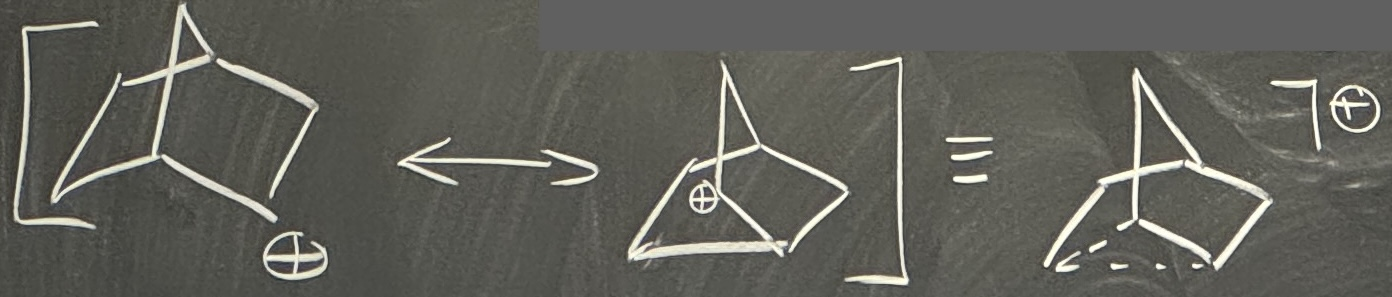
\includegraphics[width=0.9\linewidth]{nonclassicalCCa.JPG}
            \caption{3c-2e bonds.}
            \label{fig:nonclassicalCCa}
        \end{subfigure}
        \begin{subfigure}[b]{0.3\linewidth}
            \centering
            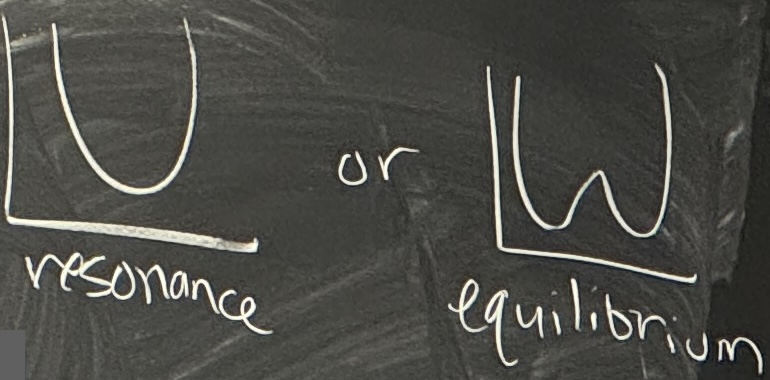
\includegraphics[width=0.8\linewidth]{nonclassicalCCb.JPG}
            \caption{Energy diagrams.}
            \label{fig:nonclassicalCCb}
        \end{subfigure}
        \caption{Nonclassical cations.}
        \label{fig:nonclassicalCC}
    \end{figure}
    \begin{itemize}
        \item Consider two cations: The $3^\circ$ \emph{tert}-butyl cation and a $2^\circ$ cation on norbornane.
        \begin{itemize}
            \item Interestingly, $\text{HIA}=\SI[per-mode=symbol]{231}{\kilo\calorie\per\mole}$ for \emph{both} of these cations!
            \item How can they both be equally stable?
        \end{itemize}
        \item This question led to the discovery of nonclassical 3c-2e bonds (Figure \ref{fig:nonclassicalCCa}).
        \begin{itemize}
            \item Essentially, we can draw two no-bond resonance forms for this cation. We move one of the $\sigma$-bonds in each of these (which we're not usually supposed to do).
            \item Thus, we can draw the real structure with two half bonds.
        \end{itemize}
        \pagebreak
        \item Aside (chemis-tea): The debate as to whether the true structure of nonclassical cations was barrierless resonance or an equilibrium between two cations raged in the literature for 70 years (Figure \ref{fig:nonclassicalCCb}).
        \begin{itemize}
            \item On team resonance: Olah (Nobel prize for this cation work), Wintsein, Schleyer, Saunder.
            \item On team equilibrium: H. C. Brown (Nobel prize for unrelated work).
            \item Brown just thought this was due to poor techniques.
            \item They would go to conferences, sit in the front row, yell at each other; publish snarky papers at each other.
            \item Debate era: 1940s-2010s.
            \item The debate ended at Science, 2013, 62 with an X-ray structure of the nonclassical cation (which really supported the resonance team). Unfortunately, H.C. Brown died in 2004. Anybody who knew Brown said he wouldn't have accepted this either.
            \item "One would have thought that the application of careful experiment and intelligent thought would lead to a rapid solution to the [nonclassical carbocation] problem. This has not been the case" - Brown's book.
            \item Until they could prove the structure of one or both, we couldn't know. This really drove the development of spectroscopy, NMR, low-temperature analysis of exotic species, etc. Essentially, people work hard when their ego is at state.
        \end{itemize}
    \end{itemize}
    \item Takeaway from our discussion of nonclassical cations: Cations exist on a spectrum.
    \begin{figure}[h!]
        \centering
        \footnotesize
        \setcharge{extra sep=5pt}
        \begin{subfigure}[b]{0.2\linewidth}
            \centering
            \chemfig{R-[:-60]-\charge{0=$\oplus$}{}}
            \caption{Most classical.}
            \label{fig:CCspectruma}
        \end{subfigure}
        \begin{subfigure}[b]{0.2\linewidth}
            \centering
            \chemfig{R-[:-80,,,,dashed]@{C1}-@{C2}\charge{0=$\oplus$}{}}
            \chemmove{
                \draw [-,dashed] ([xshift=2pt]$(C1)+(90:2pt)$) -- ($(C2)+(90:2pt)$);
            }
            \caption{Hyperconjugation.}
            \label{fig:CCspectrumb}
        \end{subfigure}
        \begin{subfigure}[b]{0.2\linewidth}
            \centering
            \chemleft{[}
                \chemfig{R?-[:-100,,,,dashed]@{C1}-@{C2}{}?[,,dashed]}
            \chemright{]^\oplus}
            \chemmove{
                \draw [-,dashed] ([xshift=2pt]$(C1)+(90:2pt)$) -- ([xshift=-1.5pt]$(C2)+(90:2pt)$);
            }
            \caption{Partial bridging.}
            \label{fig:CCspectrumc}
        \end{subfigure}
        \begin{subfigure}[b]{0.2\linewidth}
            \centering
            \chemleft{[}
                \chemfig[atom sep=2.5em]{*3([:-30]@{C1}-@{C2}-[,,,,dashed]R-[,,,,dashed])}
            \chemright{]^\oplus}
            \chemmove{
                \draw [-,dashed] ([xshift=3pt]$(C1)+(90:2pt)$) -- ([xshift=-3pt]$(C2)+(90:2pt)$);
            }
            \caption{Most nonclassical.}
            \label{fig:CCspectrumd}
        \end{subfigure}
        \caption{A spectrum of cations.}
        \label{fig:CCspectrum}
    \end{figure}
    \begin{itemize}
        \item Most classical: Discrete, trivalent, trigonal carbocations.
        \begin{itemize}
            \item These rarely exist.
        \end{itemize}
        \item Next step: Hyperconjugation and resonance.
        \begin{itemize}
            \item This accounts for most carbocations.
        \end{itemize}
        \item Next step: Some kind of bridging but asymmetric carbocation.
        \begin{itemize}
            \item There are some examples.
        \end{itemize}
        \item Most nonclassical: Bridging, symmetric carbocations (3c-2e).
        \begin{itemize}
            \item These have to be special cases, such as the norbornane one.
        \end{itemize}
    \end{itemize}
\end{itemize}




\end{document}